\chapter{Background}
\label{background}

\section{What ICSs are}
Industrial control systems (ICSs) are specialized computer systems that are used to control and monitor industrial processes. These processes can include manufacturing, power generation, water and waste management, and transportation systems. ICSs are often found in critical infrastructure facilities such as power plants, oil and gas refineries, and chemical plants.

ICSs are different from traditional IT systems in several key ways. Firstly, ICSs are designed to control physical processes, whereas IT systems are designed to process and store data. This means that ICSs have different requirements for availability, reliability, and performance. Secondly, ICSs are typically deployed in environments that are harsh and have limited resources, such as extreme temperatures and limited power. Thirdly, the protocols and hardware used in ICSs are often proprietary and not widely used outside of the industrial sector.

ICSs are becoming increasingly connected to the internet and other networks, which has led to increased concerns about their security. Industrial systems were not originally designed with security in mind, and many of them have known vulnerabilities that could be exploited by attackers. Additionally, the use of legacy systems and equipment can make it difficult to implement security measures. As a result, ICSs are increasingly seen as a potential target for cyber attacks, which could have serious consequences for the safe and reliable operation of critical infrastructure.

The increasing connectivity of ICSs and the associated security risks have led to a growing interest in the field of ICS security. Researchers and practitioners are working to develop new security technologies, standards, and best practices to protect ICSs from cyber attacks. This includes efforts to improve the security of ICS networks and devices, as well as the development of new monitoring and detection techniques to identify and respond to cyber attacks.

Supervisory Control and Data Acquisition (SCADA) systems are a type of industrial control system (ICS) that are used to remotely monitor and control industrial processes. SCADA systems are typically used in industries such as electric power generation and distribution, water and waste management, oil and gas production, and transportation systems.

SCADA systems are composed of several different components, including remote terminal units (RTUs), programmable logic controllers (PLCs), and a master station. RTUs and PLCs are used to collect data from sensors and control devices in the field, while the master station is used to display and analyze the data and make control decisions. SCADA systems also often include a human-machine interface (HMI) that is used to display process data and allow operators to interact with the system.

SCADA systems are known for their ability to monitor and control large-scale industrial processes, and for their ability to operate over long distances. This makes them well-suited for use in remote locations or for controlling processes that are spread out over a wide area. However, the same features that make SCADA systems so useful also make them vulnerable to cyber attacks.

SCADA systems were not originally designed with security in mind, and many of them have known vulnerabilities that could be exploited by attackers. Additionally, the use of legacy systems and equipment can make it difficult to implement security measures. As a result, SCADA systems are increasingly seen as a potential target for cyber attacks, which could have serious consequences for the safe and reliable operation of critical infrastructure.

To secure SCADA systems, it is important to implement security measures such as network segmentation, secure communication protocols, and access control. Additionally, it is important to monitor SCADA systems for unusual activity and to implement incident response procedures to quickly detect and respond to any security breaches.

\section{ICS components}
\label{sec:ics_components}
Industrial control systems (ICSs) are composed of several different components that work together to monitor and control industrial processes. These components include:
\begin{enumerate}

\item Field devices: These are the sensors and actuators that are used to collect data from the process and control it. Examples of field devices include temperature sensors, pressure sensors, and valves.

\item Programmable Logic Controllers (PLCs): These are specialized computers that are used to control industrial processes. PLCs are programmed with logic that defines how the process should operate and can be used to make control decisions based on data from the field devices.

\item Remote Terminal Units (RTUs): These are devices that are used to collect data from field devices and send it to the PLCs or the control center. RTUs can also be used to control field devices based on instructions from the PLCs.

\item Human-Machine Interface (HMI): This is the interface that operators use to interact with the ICS. HMIs can be used to display process data, make control decisions, and configure the ICS.

\item Supervisory Control and Data Acquisition (SCADA) systems: These are specialized systems that are used to remotely monitor and control industrial processes. SCADA systems typically include a master station that is used to display and analyze data, and make control decisions.

\item Communication Networks: These are the networks that are used to connect the different components of the ICS and allow them to communicate with each other. Communication networks can include wired and wireless networks, such as Ethernet, MODBUS, and DNP3.

\item Cybersecurity components: This can include firewalls, intrusion detection and prevention systems (IDPS), and security information and event management (SIEM) systems. These are used to protect the ICS from cyber threats and vulnerabilities.

\end{enumerate}

\subsection{RTU}
\subsection{PLC}
\subsection{IED}
\subsection{HMI}

\section{ICS Communication Protocols}
\label{sec:ics_protocols}
\subsection{Modbus}
\subsection{Ethernet/IP}
\subsection{Other Protocols}

Test cite \cite{ceccato} \\
test cite 2 \cite{itrust_swat} \\
test cite 3 \cite{itrust_site} \\
test cite 3 \cite{itrust_invariants_paper}\\

\begin{figure}[h]
	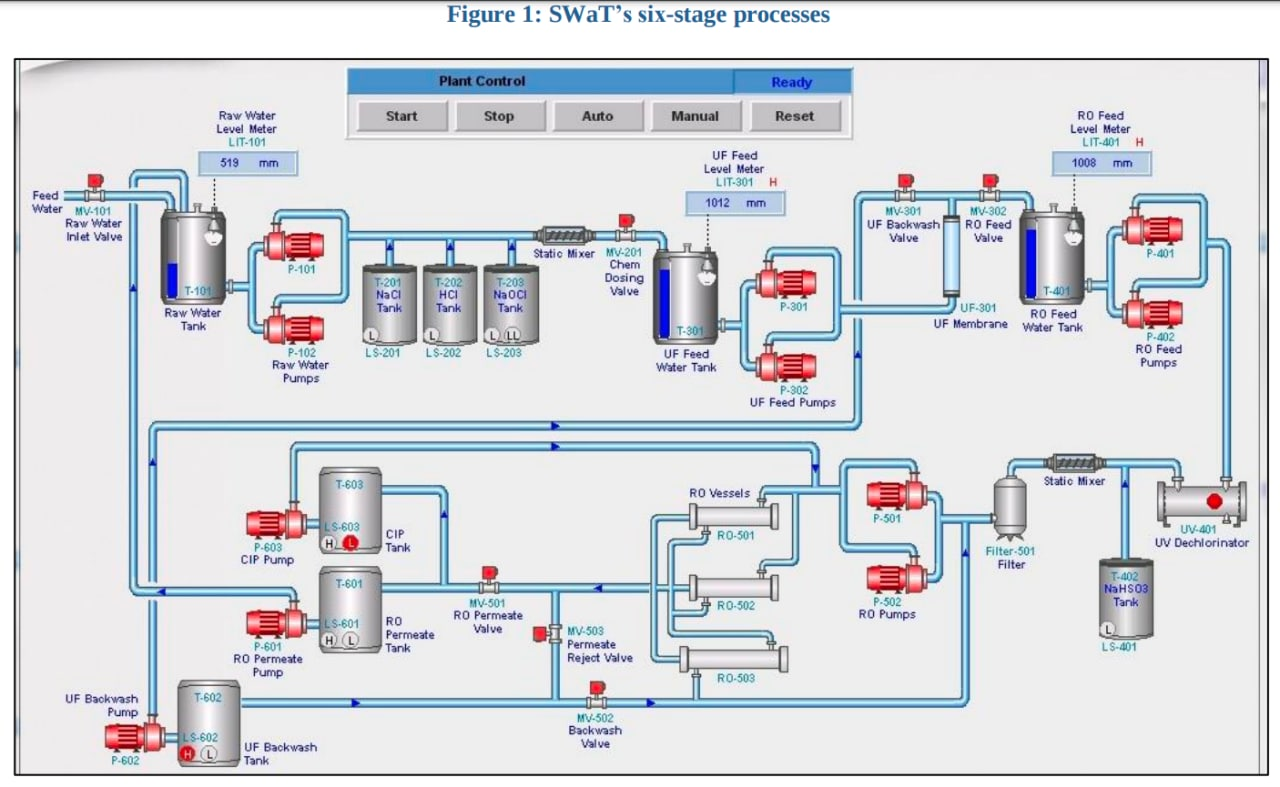
\includegraphics[scale=0.3]{swat_schema_2}
	\caption{SWaT schema}
	\label{fig:Schema SWaT}
\end{figure}

\begin{table}
	\centering
	\begin{tabular}{||c c c c||} 
		\hline
		Col1 & Col2 & Col2 & Col3 \\ [0.5ex] 
		\hline
		 & & & \\
		1 & 6 & 87837 & 787 \\ 
		2 & 7 & 78 & 5415 \\
		3 & 545 & 778 & 7507 \\
		4 & 545 & 18744 & 7560 \\
		5 & 88 & 788 & 6344 \\ [1ex] 
		\hline
	\end{tabular}
	\caption{This is the caption for the first table.}
	\label{table:1}
\end{table}
